% !TEX root = poster.tex
\node [mybox,anchor=north west, font=\fontsize{\fntszL}{\fntszL}\selectfont]
at (\chalPos) (boxChal){%
\begin{minipage}{\bxszA}

\bigskip
\bigskip
\bigskip

 Additive model discrepancy (Kennedy-O'Hagan, 2001)
 \centerline{
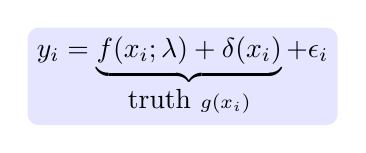
\begin{tikzpicture} \node [rounded corners,fill=blue!10] {
$y_i=\underbrace{f(x_i;\lambda)+\delta(x_i)}_{\textrm{truth } g(x_i)}+\epsilon_i$
};
\end{tikzpicture}
}
has challenges for physical models:
\begin{itemize}
%\item Calibrated prediction: $\quad f(x;\lambda)+\delta(x)\quad$ or $\quad f(x;\lambda)$ ?
\item Strong priors required on $\delta(x)$ to satisfy physical constraints
%\begin{itemize}
%\item  \emph{e.g.}  incompressible flow: $\nabla \cdot v=0$
%\end{itemize}
\item Disambiguation of model error $\delta(x_i)$ and data error $\epsilon_i$
\item $\delta(x)$ is QoI-specific; no extrapolation to other QoIs
%Calibration of model error on measured observable does not      impact the quality of model predictions on other QoIs
 %\item Physical scientists are unlikely to augment their model with a statistical model error term on select outputs
%\item Model-to-model calibration ($\epsilon_i=0$): no statistical structure of the discrepancy
\item Correlation structure in $\delta(x)$ should ideally be informed by the model $f(x;\lambda)$
\end{itemize}
\end{minipage}
};
\node[fancytitle, right=10pt, font=\fontsize{\fntszL}{\fntszL}\selectfont]
at (boxChal.north west) {\bf Model Error Challenge};
